\documentclass[1p]{elsarticle_modified}
%\bibliographystyle{elsarticle-num}

%\usepackage[colorlinks]{hyperref}
%\usepackage{abbrmath_seonhwa} %\Abb, \Ascr, \Acal ,\Abf, \Afrak
\usepackage{amsfonts}
\usepackage{amssymb}
\usepackage{amsmath}
\usepackage{amsthm}
\usepackage{scalefnt}
\usepackage{amsbsy}
\usepackage{kotex}
\usepackage{caption}
\usepackage{subfig}
\usepackage{color}
\usepackage{graphicx}
\usepackage{xcolor} %% white, black, red, green, blue, cyan, magenta, yellow
\usepackage{float}
\usepackage{setspace}
\usepackage{hyperref}

\usepackage{tikz}
\usetikzlibrary{arrows}

\usepackage{multirow}
\usepackage{array} % fixed length table
\usepackage{hhline}

%%%%%%%%%%%%%%%%%%%%%
\makeatletter
\renewcommand*\env@matrix[1][\arraystretch]{%
	\edef\arraystretch{#1}%
	\hskip -\arraycolsep
	\let\@ifnextchar\new@ifnextchar
	\array{*\c@MaxMatrixCols c}}
\makeatother %https://tex.stackexchange.com/questions/14071/how-can-i-increase-the-line-spacing-in-a-matrix
%%%%%%%%%%%%%%%

\usepackage[normalem]{ulem}

\newcommand{\msout}[1]{\ifmmode\text{\sout{\ensuremath{#1}}}\else\sout{#1}\fi}
%SOURCE: \msout is \stkout macro in https://tex.stackexchange.com/questions/20609/strikeout-in-math-mode

\newcommand{\cancel}[1]{
	\ifmmode
	{\color{red}\msout{#1}}
	\else
	{\color{red}\sout{#1}}
	\fi
}

\newcommand{\add}[1]{
	{\color{blue}\uwave{#1}}
}

\newcommand{\replace}[2]{
	\ifmmode
	{\color{red}\msout{#1}}{\color{blue}\uwave{#2}}
	\else
	{\color{red}\sout{#1}}{\color{blue}\uwave{#2}}
	\fi
}

\newcommand{\Sol}{\mathcal{S}} %segment
\newcommand{\D}{D} %diagram
\newcommand{\A}{\mathcal{A}} %arc


%%%%%%%%%%%%%%%%%%%%%%%%%%%%%5 test

\def\sl{\operatorname{\textup{SL}}(2,\Cbb)}
\def\psl{\operatorname{\textup{PSL}}(2,\Cbb)}
\def\quan{\mkern 1mu \triangleright \mkern 1mu}

\theoremstyle{definition}
\newtheorem{thm}{Theorem}[section]
\newtheorem{prop}[thm]{Proposition}
\newtheorem{lem}[thm]{Lemma}
\newtheorem{ques}[thm]{Question}
\newtheorem{cor}[thm]{Corollary}
\newtheorem{defn}[thm]{Definition}
\newtheorem{exam}[thm]{Example}
\newtheorem{rmk}[thm]{Remark}
\newtheorem{alg}[thm]{Algorithm}

\newcommand{\I}{\sqrt{-1}}
\begin{document}

%\begin{frontmatter}
%
%\title{Boundary parabolic representations of knots up to 8 crossings}
%
%%% Group authors per affiliation:
%\author{Yunhi Cho} 
%\address{Department of Mathematics, University of Seoul, Seoul, Korea}
%\ead{yhcho@uos.ac.kr}
%
%
%\author{Seonhwa Kim} %\fnref{s_kim}}
%\address{Center for Geometry and Physics, Institute for Basic Science, Pohang, 37673, Korea}
%\ead{ryeona17@ibs.re.kr}
%
%\author{Hyuk Kim}
%\address{Department of Mathematical Sciences, Seoul National University, Seoul 08826, Korea}
%\ead{hyukkim@snu.ac.kr}
%
%\author{Seokbeom Yoon}
%\address{Department of Mathematical Sciences, Seoul National University, Seoul, 08826,  Korea}
%\ead{sbyoon15@snu.ac.kr}
%
%\begin{abstract}
%We find all boundary parabolic representation of knots up to 8 crossings.
%
%\end{abstract}
%\begin{keyword}
%    \MSC[2010] 57M25 
%\end{keyword}
%
%\end{frontmatter}

%\linenumbers
%\tableofcontents
%
\newcommand\colored[1]{\textcolor{white}{\rule[-0.35ex]{0.8em}{1.4ex}}\kern-0.8em\color{red} #1}%
%\newcommand\colored[1]{\textcolor{white}{ #1}\kern-2.17ex	\textcolor{white}{ #1}\kern-1.81ex	\textcolor{white}{ #1}\kern-2.15ex\color{red}#1	}

{\Large $\underline{12a_{0840}~(K12a_{0840})}$}

\setlength{\tabcolsep}{10pt}
\renewcommand{\arraystretch}{1.6}
\vspace{1cm}\begin{tabular}{m{100pt}>{\centering\arraybackslash}m{274pt}}
\multirow{5}{120pt}{
	\centering
	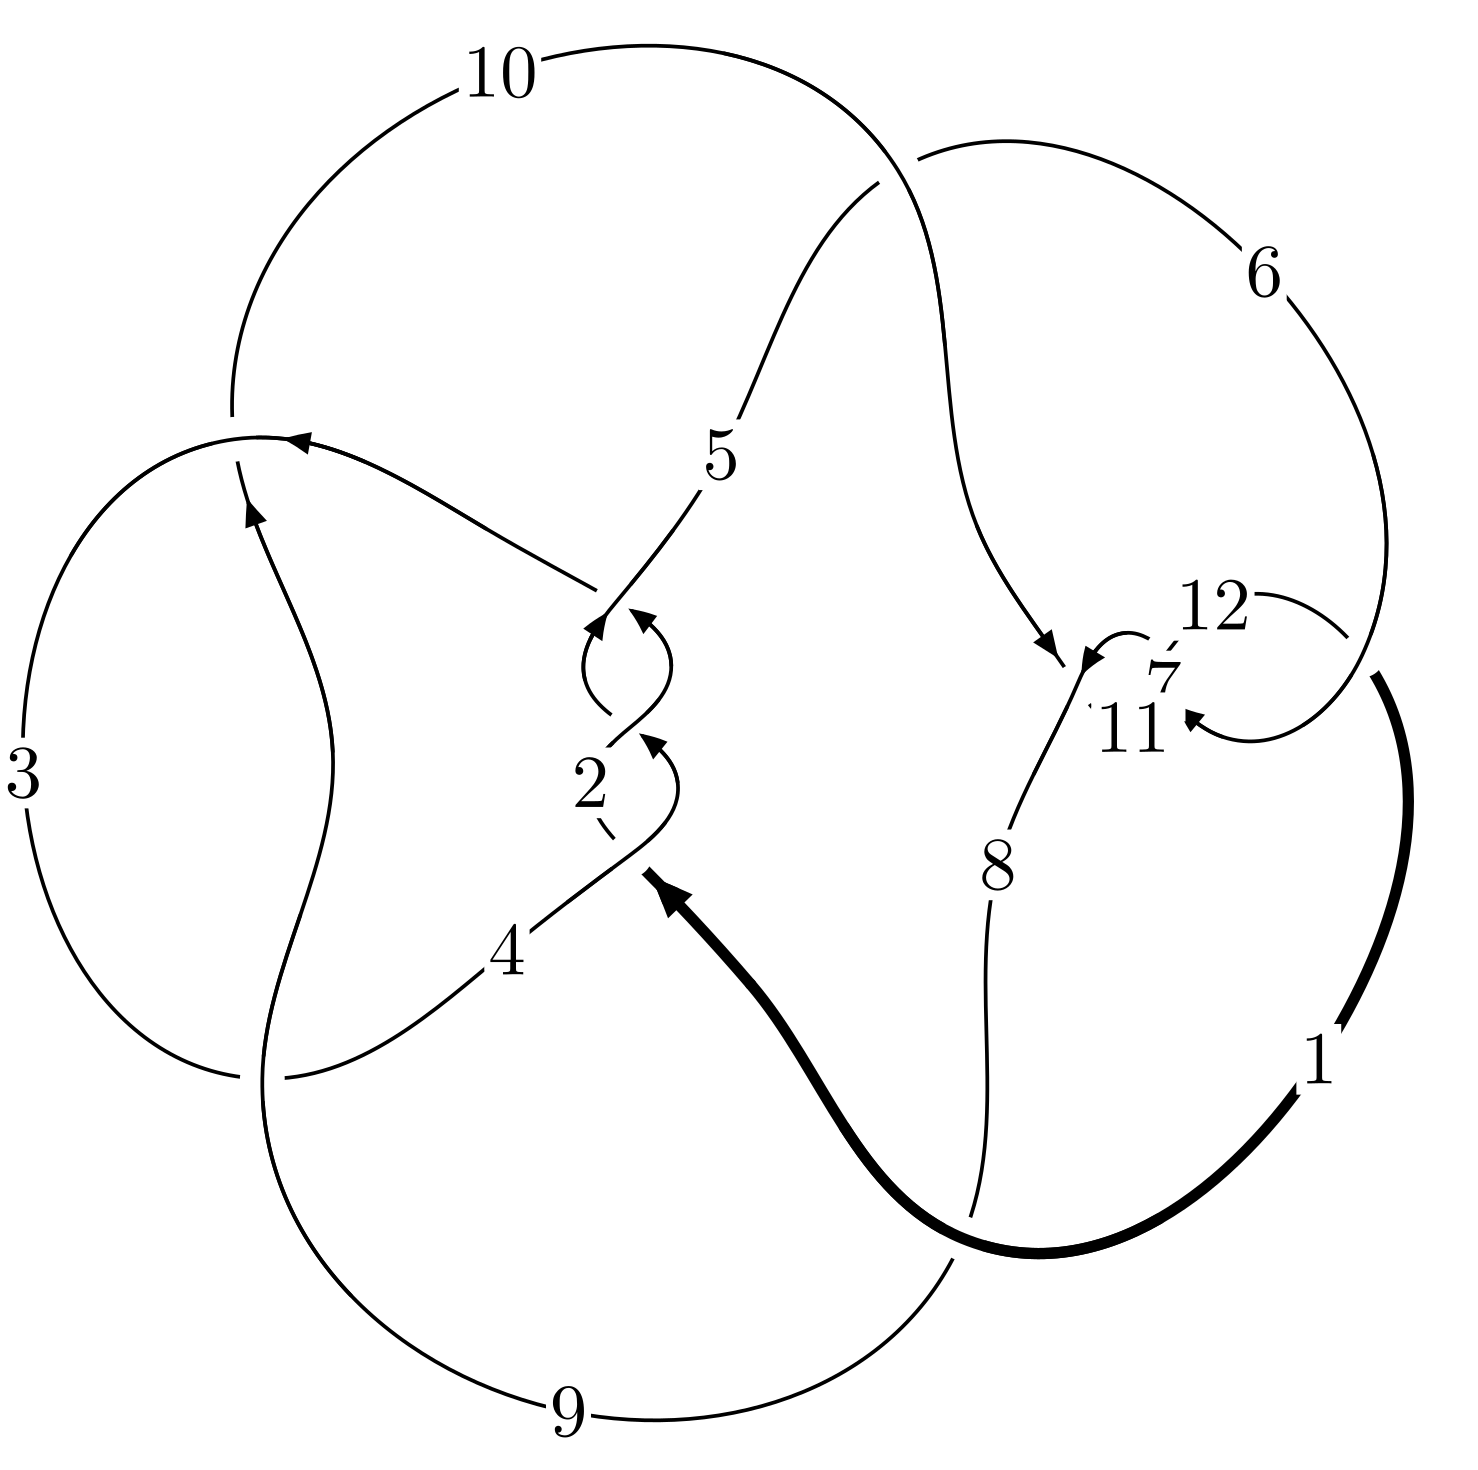
\includegraphics[width=112pt]{../../../GIT/diagram.site/Diagrams/png/1641_12a_0840.png}\\
\ \ \ A knot diagram\footnotemark}&
\allowdisplaybreaks
\textbf{Linearized knot diagam} \\
\cline{2-2}
 &
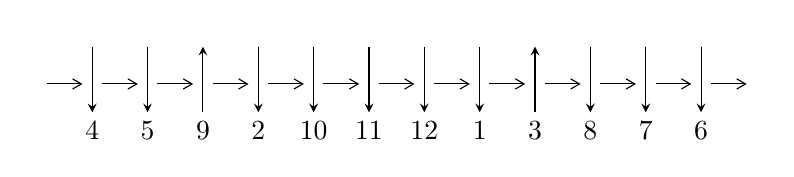
\begin{tikzpicture}[x=20pt, y=17pt]
	% nodes
	\node (C0) at (0, 0) {};
	\node (C1) at (1, 0) {};
	\node (C1U) at (1, +1) {};
	\node (C1D) at (1, -1) {4};

	\node (C2) at (2, 0) {};
	\node (C2U) at (2, +1) {};
	\node (C2D) at (2, -1) {5};

	\node (C3) at (3, 0) {};
	\node (C3U) at (3, +1) {};
	\node (C3D) at (3, -1) {9};

	\node (C4) at (4, 0) {};
	\node (C4U) at (4, +1) {};
	\node (C4D) at (4, -1) {2};

	\node (C5) at (5, 0) {};
	\node (C5U) at (5, +1) {};
	\node (C5D) at (5, -1) {10};

	\node (C6) at (6, 0) {};
	\node (C6U) at (6, +1) {};
	\node (C6D) at (6, -1) {11};

	\node (C7) at (7, 0) {};
	\node (C7U) at (7, +1) {};
	\node (C7D) at (7, -1) {12};

	\node (C8) at (8, 0) {};
	\node (C8U) at (8, +1) {};
	\node (C8D) at (8, -1) {1};

	\node (C9) at (9, 0) {};
	\node (C9U) at (9, +1) {};
	\node (C9D) at (9, -1) {3};

	\node (C10) at (10, 0) {};
	\node (C10U) at (10, +1) {};
	\node (C10D) at (10, -1) {8};

	\node (C11) at (11, 0) {};
	\node (C11U) at (11, +1) {};
	\node (C11D) at (11, -1) {7};

	\node (C12) at (12, 0) {};
	\node (C12U) at (12, +1) {};
	\node (C12D) at (12, -1) {6};
	\node (C13) at (13, 0) {};

	% arrows
	\draw[->,>={angle 60}]
	(C0) edge (C1) (C1) edge (C2) (C2) edge (C3) (C3) edge (C4) (C4) edge (C5) (C5) edge (C6) (C6) edge (C7) (C7) edge (C8) (C8) edge (C9) (C9) edge (C10) (C10) edge (C11) (C11) edge (C12) (C12) edge (C13) ;	\draw[->,>=stealth]
	(C1U) edge (C1D) (C2U) edge (C2D) (C3D) edge (C3U) (C4U) edge (C4D) (C5U) edge (C5D) (C6U) edge (C6D) (C7U) edge (C7D) (C8U) edge (C8D) (C9D) edge (C9U) (C10U) edge (C10D) (C11U) edge (C11D) (C12U) edge (C12D) ;
	\end{tikzpicture} \\
\hhline{~~} \\& 
\textbf{Solving Sequence} \\ \cline{2-2} 
 &
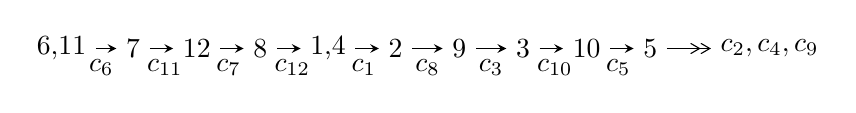
\begin{tikzpicture}[x=23pt, y=7pt]
	% node
	\node (A0) at (-1/8, 0) {6,11};
	\node (A1) at (1, 0) {7};
	\node (A2) at (2, 0) {12};
	\node (A3) at (3, 0) {8};
	\node (A4) at (65/16, 0) {1,4};
	\node (A5) at (41/8, 0) {2};
	\node (A6) at (49/8, 0) {9};
	\node (A7) at (57/8, 0) {3};
	\node (A8) at (65/8, 0) {10};
	\node (A9) at (73/8, 0) {5};
	\node (C1) at (1/2, -1) {$c_{6}$};
	\node (C2) at (3/2, -1) {$c_{11}$};
	\node (C3) at (5/2, -1) {$c_{7}$};
	\node (C4) at (7/2, -1) {$c_{12}$};
	\node (C5) at (37/8, -1) {$c_{1}$};
	\node (C6) at (45/8, -1) {$c_{8}$};
	\node (C7) at (53/8, -1) {$c_{3}$};
	\node (C8) at (61/8, -1) {$c_{10}$};
	\node (C9) at (69/8, -1) {$c_{5}$};
	\node (A10) at (11, 0) {$c_{2},c_{4},c_{9}$};

	% edge
	\draw[->,>=stealth]	
	(A0) edge (A1) (A1) edge (A2) (A2) edge (A3) (A3) edge (A4) (A4) edge (A5) (A5) edge (A6) (A6) edge (A7) (A7) edge (A8) (A8) edge (A9) ;
	\draw[->>,>={angle 60}]	
	(A9) edge (A10);
\end{tikzpicture} \\ 

\end{tabular} \\

\footnotetext{
The image of knot diagram is generated by the software ``\textbf{Draw programme}" developed by Andrew Bartholomew(\url{http://www.layer8.co.uk/maths/draw/index.htm\#Running-draw}), where we modified some parts for our purpose(\url{https://github.com/CATsTAILs/LinksPainter}).
}\phantom \\ \newline 
\centering \textbf{Ideals for irreducible components\footnotemark of $X_{\text{par}}$} 
 
\begin{align*}
I^u_{1}&=\langle 
u^{70}+u^{69}+\cdots+b+2 u,\;u^{70}+u^{69}+\cdots+a+8 u,\;u^{71}+2 u^{70}+\cdots+10 u^2-1\rangle \\
I^u_{2}&=\langle 
b+1,\;u^6-3 u^4+u^3+2 u^2+a-2 u+1,\;u^8+u^7-3 u^6-2 u^5+3 u^4+2 u-1\rangle \\
\\
\end{align*}
\raggedright * 2 irreducible components of $\dim_{\mathbb{C}}=0$, with total 79 representations.\\
\footnotetext{All coefficients of polynomials are rational numbers. But the coefficients are sometimes approximated in decimal forms when there is not enough margin.}
\newpage
\renewcommand{\arraystretch}{1}
\centering \section*{I. $I^u_{1}= \langle u^{70}+u^{69}+\cdots+b+2 u,\;u^{70}+u^{69}+\cdots+a+8 u,\;u^{71}+2 u^{70}+\cdots+10 u^2-1 \rangle$}
\flushleft \textbf{(i) Arc colorings}\\
\begin{tabular}{m{7pt} m{180pt} m{7pt} m{180pt} }
\flushright $a_{6}=$&$\begin{pmatrix}1\\0\end{pmatrix}$ \\
\flushright $a_{11}=$&$\begin{pmatrix}0\\u\end{pmatrix}$ \\
\flushright $a_{7}=$&$\begin{pmatrix}1\\u^2\end{pmatrix}$ \\
\flushright $a_{12}=$&$\begin{pmatrix}- u\\- u^3+u\end{pmatrix}$ \\
\flushright $a_{8}=$&$\begin{pmatrix}- u^2+1\\- u^4+2 u^2\end{pmatrix}$ \\
\flushright $a_{1}=$&$\begin{pmatrix}u^3-2 u\\- u^3+u\end{pmatrix}$ \\
\flushright $a_{4}=$&$\begin{pmatrix}- u^{70}- u^{69}+\cdots-20 u^2-8 u\\- u^{70}- u^{69}+\cdots-9 u^2-2 u\end{pmatrix}$ \\
\flushright $a_{2}=$&$\begin{pmatrix}-2 u^{70}-2 u^{69}+\cdots-22 u^2-9 u\\- u^{70}- u^{69}+\cdots-9 u^2-2 u\end{pmatrix}$ \\
\flushright $a_{9}=$&$\begin{pmatrix}u^{10}-5 u^8+8 u^6-3 u^4-3 u^2+1\\- u^{10}+4 u^8-5 u^6+3 u^2\end{pmatrix}$ \\
\flushright $a_{3}=$&$\begin{pmatrix}-3 u^{70}-3 u^{69}+\cdots-8 u+1\\- u^{70}- u^{69}+\cdots-10 u^2-3 u\end{pmatrix}$ \\
\flushright $a_{10}=$&$\begin{pmatrix}u^5-2 u^3+u\\u^7-3 u^5+2 u^3+u\end{pmatrix}$ \\
\flushright $a_{5}=$&$\begin{pmatrix}- u^{12}+5 u^{10}-9 u^8+6 u^6- u^2+1\\- u^{14}+6 u^{12}-13 u^{10}+10 u^8+2 u^6-4 u^4- u^2\end{pmatrix}$\\&\end{tabular}
\flushleft \textbf{(ii) Obstruction class $= -1$}\\~\\
\flushleft \textbf{(iii) Cusp Shapes $= u^{70}+4 u^{69}+\cdots+10 u-5$}\\~\\
\newpage\renewcommand{\arraystretch}{1}
\flushleft \textbf{(iv) u-Polynomials at the component}\newline \\
\begin{tabular}{m{50pt}|m{274pt}}
Crossings & \hspace{64pt}u-Polynomials at each crossing \\
\hline $$\begin{aligned}c_{1},c_{2},c_{4}\end{aligned}$$&$\begin{aligned}
&u^{71}-9 u^{70}+\cdots-8 u+1
\end{aligned}$\\
\hline $$\begin{aligned}c_{3},c_{9}\end{aligned}$$&$\begin{aligned}
&u^{71}- u^{70}+\cdots+896 u+256
\end{aligned}$\\
\hline $$\begin{aligned}c_{5},c_{8}\end{aligned}$$&$\begin{aligned}
&u^{71}-2 u^{70}+\cdots+1648 u-505
\end{aligned}$\\
\hline $$\begin{aligned}c_{6},c_{7},c_{11}\end{aligned}$$&$\begin{aligned}
&u^{71}+2 u^{70}+\cdots+10 u^2-1
\end{aligned}$\\
\hline $$\begin{aligned}c_{10},c_{12}\end{aligned}$$&$\begin{aligned}
&u^{71}-6 u^{70}+\cdots-4 u+1
\end{aligned}$\\
\hline
\end{tabular}\\~\\
\newpage\renewcommand{\arraystretch}{1}
\flushleft \textbf{(v) Riley Polynomials at the component}\newline \\
\begin{tabular}{m{50pt}|m{274pt}}
Crossings & \hspace{64pt}Riley Polynomials at each crossing \\
\hline $$\begin{aligned}c_{1},c_{2},c_{4}\end{aligned}$$&$\begin{aligned}
&y^{71}-73 y^{70}+\cdots+40 y-1
\end{aligned}$\\
\hline $$\begin{aligned}c_{3},c_{9}\end{aligned}$$&$\begin{aligned}
&y^{71}+51 y^{70}+\cdots+376832 y-65536
\end{aligned}$\\
\hline $$\begin{aligned}c_{5},c_{8}\end{aligned}$$&$\begin{aligned}
&y^{71}-60 y^{70}+\cdots+2629044 y-255025
\end{aligned}$\\
\hline $$\begin{aligned}c_{6},c_{7},c_{11}\end{aligned}$$&$\begin{aligned}
&y^{71}-60 y^{70}+\cdots+20 y-1
\end{aligned}$\\
\hline $$\begin{aligned}c_{10},c_{12}\end{aligned}$$&$\begin{aligned}
&y^{71}+36 y^{70}+\cdots+20 y-1
\end{aligned}$\\
\hline
\end{tabular}\\~\\
\newpage\flushleft \textbf{(vi) Complex Volumes and Cusp Shapes}
$$\begin{array}{c|c|c}  
\text{Solutions to }I^u_{1}& \I (\text{vol} + \sqrt{-1}CS) & \text{Cusp shape}\\
 \hline 
\begin{aligned}
u &= \phantom{-}0.986659 + 0.246337 I \\
a &= \phantom{-}0.840333 + 0.355711 I \\
b &= -0.851935 + 0.777616 I\end{aligned}
 & -4.39759 + 2.62166 I & -12.54325 + 0. I\phantom{ +0.000000I} \\ \hline\begin{aligned}
u &= \phantom{-}0.986659 - 0.246337 I \\
a &= \phantom{-}0.840333 - 0.355711 I \\
b &= -0.851935 - 0.777616 I\end{aligned}
 & -4.39759 - 2.62166 I & -12.54325 + 0. I\phantom{ +0.000000I} \\ \hline\begin{aligned}
u &= \phantom{-}0.996077 + 0.329643 I \\
a &= -2.15290 - 1.03284 I \\
b &= \phantom{-}2.27588 - 0.46222 I\end{aligned}
 & -11.10650 + 6.59599 I & \phantom{-0.000000 } 0 \\ \hline\begin{aligned}
u &= \phantom{-}0.996077 - 0.329643 I \\
a &= -2.15290 + 1.03284 I \\
b &= \phantom{-}2.27588 + 0.46222 I\end{aligned}
 & -11.10650 - 6.59599 I & \phantom{-0.000000 } 0 \\ \hline\begin{aligned}
u &= -0.908611 + 0.214665 I \\
a &= -2.60723 + 0.20772 I \\
b &= \phantom{-}1.91874 + 0.49065 I\end{aligned}
 & -6.64883 - 0.06384 I & -13.96488 - 0.64877 I \\ \hline\begin{aligned}
u &= -0.908611 - 0.214665 I \\
a &= -2.60723 - 0.20772 I \\
b &= \phantom{-}1.91874 - 0.49065 I\end{aligned}
 & -6.64883 + 0.06384 I & -13.96488 + 0.64877 I \\ \hline\begin{aligned}
u &= \phantom{-}0.809385 + 0.207067 I \\
a &= \phantom{-}0.362023 - 0.291325 I \\
b &= -0.557314 - 0.483316 I\end{aligned}
 & -4.57830 - 2.54230 I & -13.6596 + 4.1821 I \\ \hline\begin{aligned}
u &= \phantom{-}0.809385 - 0.207067 I \\
a &= \phantom{-}0.362023 + 0.291325 I \\
b &= -0.557314 + 0.483316 I\end{aligned}
 & -4.57830 + 2.54230 I & -13.6596 - 4.1821 I \\ \hline\begin{aligned}
u &= \phantom{-}0.766372 + 0.323559 I \\
a &= -1.75720 + 0.29981 I \\
b &= \phantom{-}1.83541 - 0.37016 I\end{aligned}
 & -11.57750 - 6.28991 I & -15.1916 + 4.8659 I \\ \hline\begin{aligned}
u &= \phantom{-}0.766372 - 0.323559 I \\
a &= -1.75720 - 0.29981 I \\
b &= \phantom{-}1.83541 + 0.37016 I\end{aligned}
 & -11.57750 + 6.28991 I & -15.1916 - 4.8659 I\\
 \hline 
 \end{array}$$\newpage$$\begin{array}{c|c|c}  
\text{Solutions to }I^u_{1}& \I (\text{vol} + \sqrt{-1}CS) & \text{Cusp shape}\\
 \hline 
\begin{aligned}
u &= -1.154890 + 0.240784 I \\
a &= \phantom{-}0.924878 + 0.182653 I \\
b &= -0.298204 - 0.725011 I\end{aligned}
 & -1.31391 + 0.68641 I & \phantom{-0.000000 } 0 \\ \hline\begin{aligned}
u &= -1.154890 - 0.240784 I \\
a &= \phantom{-}0.924878 - 0.182653 I \\
b &= -0.298204 + 0.725011 I\end{aligned}
 & -1.31391 - 0.68641 I & \phantom{-0.000000 } 0 \\ \hline\begin{aligned}
u &= \phantom{-}0.181853 + 0.789212 I \\
a &= -3.78833 - 2.50123 I \\
b &= \phantom{-}2.82607 + 0.74359 I\end{aligned}
 & -8.59298 - 10.74520 I & -11.21931 + 6.66626 I \\ \hline\begin{aligned}
u &= \phantom{-}0.181853 - 0.789212 I \\
a &= -3.78833 + 2.50123 I \\
b &= \phantom{-}2.82607 - 0.74359 I\end{aligned}
 & -8.59298 + 10.74520 I & -11.21931 - 6.66626 I \\ \hline\begin{aligned}
u &= -0.066855 + 0.801312 I \\
a &= \phantom{-}1.80010 - 0.25938 I \\
b &= -1.259410 - 0.508282 I\end{aligned}
 & -1.15216 + 4.20230 I & -9.31977 - 4.21160 I \\ \hline\begin{aligned}
u &= -0.066855 - 0.801312 I \\
a &= \phantom{-}1.80010 + 0.25938 I \\
b &= -1.259410 + 0.508282 I\end{aligned}
 & -1.15216 - 4.20230 I & -9.31977 + 4.21160 I \\ \hline\begin{aligned}
u &= \phantom{-}0.176589 + 0.764676 I \\
a &= \phantom{-}1.26518 + 1.55971 I \\
b &= -1.31967 - 0.80362 I\end{aligned}
 & -1.90510 - 6.52099 I & -9.14939 + 6.60717 I \\ \hline\begin{aligned}
u &= \phantom{-}0.176589 - 0.764676 I \\
a &= \phantom{-}1.26518 - 1.55971 I \\
b &= -1.31967 + 0.80362 I\end{aligned}
 & -1.90510 + 6.52099 I & -9.14939 - 6.60717 I \\ \hline\begin{aligned}
u &= -0.185138 + 0.751263 I \\
a &= -3.20382 + 3.96451 I \\
b &= \phantom{-}2.40680 - 1.58953 I\end{aligned}
 & -4.30951 + 3.86319 I & -10.53421 - 3.73969 I \\ \hline\begin{aligned}
u &= -0.185138 - 0.751263 I \\
a &= -3.20382 - 3.96451 I \\
b &= \phantom{-}2.40680 + 1.58953 I\end{aligned}
 & -4.30951 - 3.86319 I & -10.53421 + 3.73969 I\\
 \hline 
 \end{array}$$\newpage$$\begin{array}{c|c|c}  
\text{Solutions to }I^u_{1}& \I (\text{vol} + \sqrt{-1}CS) & \text{Cusp shape}\\
 \hline 
\begin{aligned}
u &= -1.23414\phantom{ +0.000000I} \\
a &= -2.32831\phantom{ +0.000000I} \\
b &= -0.376389\phantom{ +0.000000I}\end{aligned}
 & -6.28970\phantom{ +0.000000I} & \phantom{-0.000000 } 0 \\ \hline\begin{aligned}
u &= -1.190850 + 0.346873 I \\
a &= \phantom{-}0.457682 - 0.424063 I \\
b &= -1.37788 + 0.35953 I\end{aligned}
 & -4.59392 - 0.04944 I & \phantom{-0.000000 } 0 \\ \hline\begin{aligned}
u &= -1.190850 - 0.346873 I \\
a &= \phantom{-}0.457682 + 0.424063 I \\
b &= -1.37788 - 0.35953 I\end{aligned}
 & -4.59392 + 0.04944 I & \phantom{-0.000000 } 0 \\ \hline\begin{aligned}
u &= \phantom{-}1.239300 + 0.109593 I \\
a &= \phantom{-}0.445590 - 0.103058 I \\
b &= -0.159999 - 0.708388 I\end{aligned}
 & -4.58430 - 2.00294 I & \phantom{-0.000000 } 0 \\ \hline\begin{aligned}
u &= \phantom{-}1.239300 - 0.109593 I \\
a &= \phantom{-}0.445590 + 0.103058 I \\
b &= -0.159999 + 0.708388 I\end{aligned}
 & -4.58430 + 2.00294 I & \phantom{-0.000000 } 0 \\ \hline\begin{aligned}
u &= \phantom{-}0.186710 + 0.731693 I \\
a &= \phantom{-}0.677426 + 0.479857 I \\
b &= -0.176307 + 0.203264 I\end{aligned}
 & -2.39470 - 1.09775 I & -10.39559 + 0.93933 I \\ \hline\begin{aligned}
u &= \phantom{-}0.186710 - 0.731693 I \\
a &= \phantom{-}0.677426 - 0.479857 I \\
b &= -0.176307 - 0.203264 I\end{aligned}
 & -2.39470 + 1.09775 I & -10.39559 - 0.93933 I \\ \hline\begin{aligned}
u &= -0.129455 + 0.743382 I \\
a &= \phantom{-}0.91484 - 1.53124 I \\
b &= -0.739107 + 0.752454 I\end{aligned}
 & \phantom{-}1.69012 + 2.95686 I & -2.27360 - 4.11680 I \\ \hline\begin{aligned}
u &= -0.129455 - 0.743382 I \\
a &= \phantom{-}0.91484 + 1.53124 I \\
b &= -0.739107 - 0.752454 I\end{aligned}
 & \phantom{-}1.69012 - 2.95686 I & -2.27360 + 4.11680 I \\ \hline\begin{aligned}
u &= \phantom{-}0.232613 + 0.714723 I \\
a &= -1.49386 - 3.33234 I \\
b &= \phantom{-}1.33349 + 1.10636 I\end{aligned}
 & -9.77913 + 2.47980 I & -12.49777 + 0.44362 I\\
 \hline 
 \end{array}$$\newpage$$\begin{array}{c|c|c}  
\text{Solutions to }I^u_{1}& \I (\text{vol} + \sqrt{-1}CS) & \text{Cusp shape}\\
 \hline 
\begin{aligned}
u &= \phantom{-}0.232613 - 0.714723 I \\
a &= -1.49386 + 3.33234 I \\
b &= \phantom{-}1.33349 - 1.10636 I\end{aligned}
 & -9.77913 - 2.47980 I & -12.49777 - 0.44362 I \\ \hline\begin{aligned}
u &= -0.038065 + 0.746925 I \\
a &= -1.26831 - 0.69126 I \\
b &= \phantom{-}1.057950 + 0.468795 I\end{aligned}
 & \phantom{-}3.58845 + 2.01767 I & -2.00784 - 4.42424 I \\ \hline\begin{aligned}
u &= -0.038065 - 0.746925 I \\
a &= -1.26831 + 0.69126 I \\
b &= \phantom{-}1.057950 - 0.468795 I\end{aligned}
 & \phantom{-}3.58845 - 2.01767 I & -2.00784 + 4.42424 I \\ \hline\begin{aligned}
u &= -1.234340 + 0.297863 I \\
a &= \phantom{-}0.077706 + 0.925364 I \\
b &= \phantom{-}1.063820 - 0.074072 I\end{aligned}
 & -0.08058 + 1.76105 I & \phantom{-0.000000 } 0 \\ \hline\begin{aligned}
u &= -1.234340 - 0.297863 I \\
a &= \phantom{-}0.077706 - 0.925364 I \\
b &= \phantom{-}1.063820 + 0.074072 I\end{aligned}
 & -0.08058 - 1.76105 I & \phantom{-0.000000 } 0 \\ \hline\begin{aligned}
u &= \phantom{-}1.263550 + 0.265912 I \\
a &= \phantom{-}1.184650 + 0.148415 I \\
b &= -1.40923 + 0.68906 I\end{aligned}
 & -3.14372 - 2.42246 I & \phantom{-0.000000 } 0 \\ \hline\begin{aligned}
u &= \phantom{-}1.263550 - 0.265912 I \\
a &= \phantom{-}1.184650 - 0.148415 I \\
b &= -1.40923 - 0.68906 I\end{aligned}
 & -3.14372 + 2.42246 I & \phantom{-0.000000 } 0 \\ \hline\begin{aligned}
u &= \phantom{-}0.029470 + 0.697447 I \\
a &= \phantom{-}2.38285 + 1.53386 I \\
b &= -1.62005 - 0.27761 I\end{aligned}
 & \phantom{-}0.662530 - 1.041100 I & -7.27548 - 0.38248 I \\ \hline\begin{aligned}
u &= \phantom{-}0.029470 - 0.697447 I \\
a &= \phantom{-}2.38285 - 1.53386 I \\
b &= -1.62005 + 0.27761 I\end{aligned}
 & \phantom{-}0.662530 + 1.041100 I & -7.27548 + 0.38248 I \\ \hline\begin{aligned}
u &= -1.291470 + 0.286170 I \\
a &= \phantom{-}0.10379 - 2.25863 I \\
b &= -1.84247 - 0.07524 I\end{aligned}
 & -3.46345 + 4.60561 I & \phantom{-0.000000 } 0\\
 \hline 
 \end{array}$$\newpage$$\begin{array}{c|c|c}  
\text{Solutions to }I^u_{1}& \I (\text{vol} + \sqrt{-1}CS) & \text{Cusp shape}\\
 \hline 
\begin{aligned}
u &= -1.291470 - 0.286170 I \\
a &= \phantom{-}0.10379 + 2.25863 I \\
b &= -1.84247 + 0.07524 I\end{aligned}
 & -3.46345 - 4.60561 I & \phantom{-0.000000 } 0 \\ \hline\begin{aligned}
u &= \phantom{-}1.289160 + 0.314090 I \\
a &= -0.647097 - 0.468432 I \\
b &= \phantom{-}1.042920 - 0.815117 I\end{aligned}
 & -0.54813 - 5.85187 I & \phantom{-0.000000 } 0 \\ \hline\begin{aligned}
u &= \phantom{-}1.289160 - 0.314090 I \\
a &= -0.647097 + 0.468432 I \\
b &= \phantom{-}1.042920 + 0.815117 I\end{aligned}
 & -0.54813 + 5.85187 I & \phantom{-0.000000 } 0 \\ \hline\begin{aligned}
u &= \phantom{-}1.306420 + 0.349875 I \\
a &= \phantom{-}0.68982 + 1.42591 I \\
b &= -1.128250 + 0.646449 I\end{aligned}
 & -5.44295 - 8.34894 I & \phantom{-0.000000 } 0 \\ \hline\begin{aligned}
u &= \phantom{-}1.306420 - 0.349875 I \\
a &= \phantom{-}0.68982 - 1.42591 I \\
b &= -1.128250 - 0.646449 I\end{aligned}
 & -5.44295 + 8.34894 I & \phantom{-0.000000 } 0 \\ \hline\begin{aligned}
u &= \phantom{-}1.358380 + 0.152222 I \\
a &= -1.17648 + 1.28390 I \\
b &= -1.337860 - 0.349570 I\end{aligned}
 & -11.76690 - 3.60144 I & \phantom{-0.000000 } 0 \\ \hline\begin{aligned}
u &= \phantom{-}1.358380 - 0.152222 I \\
a &= -1.17648 - 1.28390 I \\
b &= -1.337860 + 0.349570 I\end{aligned}
 & -11.76690 + 3.60144 I & \phantom{-0.000000 } 0 \\ \hline\begin{aligned}
u &= \phantom{-}1.344140 + 0.315904 I \\
a &= -0.347097 + 1.182250 I \\
b &= -0.972415 - 0.773651 I\end{aligned}
 & -2.95246 - 6.79976 I & \phantom{-0.000000 } 0 \\ \hline\begin{aligned}
u &= \phantom{-}1.344140 - 0.315904 I \\
a &= -0.347097 - 1.182250 I \\
b &= -0.972415 + 0.773651 I\end{aligned}
 & -2.95246 + 6.79976 I & \phantom{-0.000000 } 0 \\ \hline\begin{aligned}
u &= \phantom{-}1.38516\phantom{ +0.000000I} \\
a &= -0.406375\phantom{ +0.000000I} \\
b &= -1.07210\phantom{ +0.000000I}\end{aligned}
 & -7.07702\phantom{ +0.000000I} & \phantom{-0.000000 } 0\\
 \hline 
 \end{array}$$\newpage$$\begin{array}{c|c|c}  
\text{Solutions to }I^u_{1}& \I (\text{vol} + \sqrt{-1}CS) & \text{Cusp shape}\\
 \hline 
\begin{aligned}
u &= -1.367690 + 0.306384 I \\
a &= \phantom{-}0.230808 - 0.686573 I \\
b &= -0.0933768 + 0.0315903 I\end{aligned}
 & -7.30405 + 4.87123 I & \phantom{-0.000000 } 0 \\ \hline\begin{aligned}
u &= -1.367690 - 0.306384 I \\
a &= \phantom{-}0.230808 + 0.686573 I \\
b &= -0.0933768 - 0.0315903 I\end{aligned}
 & -7.30405 - 4.87123 I & \phantom{-0.000000 } 0 \\ \hline\begin{aligned}
u &= -1.367790 + 0.321539 I \\
a &= -0.393117 - 1.350420 I \\
b &= -1.56646 + 0.71385 I\end{aligned}
 & -6.78407 + 10.45570 I & \phantom{-0.000000 } 0 \\ \hline\begin{aligned}
u &= -1.367790 - 0.321539 I \\
a &= -0.393117 + 1.350420 I \\
b &= -1.56646 - 0.71385 I\end{aligned}
 & -6.78407 - 10.45570 I & \phantom{-0.000000 } 0 \\ \hline\begin{aligned}
u &= \phantom{-}1.369780 + 0.314519 I \\
a &= \phantom{-}0.49273 - 3.43980 I \\
b &= \phantom{-}2.88614 + 1.93089 I\end{aligned}
 & -9.22312 - 7.72882 I & \phantom{-0.000000 } 0 \\ \hline\begin{aligned}
u &= \phantom{-}1.369780 - 0.314519 I \\
a &= \phantom{-}0.49273 + 3.43980 I \\
b &= \phantom{-}2.88614 - 1.93089 I\end{aligned}
 & -9.22312 + 7.72882 I & \phantom{-0.000000 } 0 \\ \hline\begin{aligned}
u &= -0.396518 + 0.441005 I \\
a &= \phantom{-}0.47669 - 1.49811 I \\
b &= -1.328800 + 0.023293 I\end{aligned}
 & -6.36129 + 1.57513 I & -13.7151 - 4.1754 I \\ \hline\begin{aligned}
u &= -0.396518 - 0.441005 I \\
a &= \phantom{-}0.47669 + 1.49811 I \\
b &= -1.328800 - 0.023293 I\end{aligned}
 & -6.36129 - 1.57513 I & -13.7151 + 4.1754 I \\ \hline\begin{aligned}
u &= -1.381840 + 0.290987 I \\
a &= \phantom{-}0.90571 + 2.40675 I \\
b &= \phantom{-}1.44667 - 1.68893 I\end{aligned}
 & -14.8854 + 1.1709 I & \phantom{-0.000000 } 0 \\ \hline\begin{aligned}
u &= -1.381840 - 0.290987 I \\
a &= \phantom{-}0.90571 - 2.40675 I \\
b &= \phantom{-}1.44667 + 1.68893 I\end{aligned}
 & -14.8854 - 1.1709 I & \phantom{-0.000000 } 0\\
 \hline 
 \end{array}$$\newpage$$\begin{array}{c|c|c}  
\text{Solutions to }I^u_{1}& \I (\text{vol} + \sqrt{-1}CS) & \text{Cusp shape}\\
 \hline 
\begin{aligned}
u &= -1.373550 + 0.332446 I \\
a &= -0.39571 + 3.13248 I \\
b &= \phantom{-}3.20219 - 0.78644 I\end{aligned}
 & -13.5094 + 14.8002 I & \phantom{-0.000000 } 0 \\ \hline\begin{aligned}
u &= -1.373550 - 0.332446 I \\
a &= -0.39571 - 3.13248 I \\
b &= \phantom{-}3.20219 + 0.78644 I\end{aligned}
 & -13.5094 - 14.8002 I & \phantom{-0.000000 } 0 \\ \hline\begin{aligned}
u &= -1.41996 + 0.01011 I \\
a &= -0.416396 + 0.543396 I \\
b &= -0.966187 + 0.001876 I\end{aligned}
 & -11.25150 + 2.82348 I & \phantom{-0.000000 } 0 \\ \hline\begin{aligned}
u &= -1.41996 - 0.01011 I \\
a &= -0.416396 - 0.543396 I \\
b &= -0.966187 - 0.001876 I\end{aligned}
 & -11.25150 - 2.82348 I & \phantom{-0.000000 } 0 \\ \hline\begin{aligned}
u &= \phantom{-}1.42247\phantom{ +0.000000I} \\
a &= \phantom{-}0.946420\phantom{ +0.000000I} \\
b &= \phantom{-}3.55445\phantom{ +0.000000I}\end{aligned}
 & -13.4469\phantom{ +0.000000I} & \phantom{-0.000000 } 0 \\ \hline\begin{aligned}
u &= -1.43211 + 0.02678 I \\
a &= \phantom{-}0.860128 + 0.073018 I \\
b &= \phantom{-}2.85973 + 0.70323 I\end{aligned}
 & -18.4145 + 6.9595 I & \phantom{-0.000000 } 0 \\ \hline\begin{aligned}
u &= -1.43211 - 0.02678 I \\
a &= \phantom{-}0.860128 - 0.073018 I \\
b &= \phantom{-}2.85973 - 0.70323 I\end{aligned}
 & -18.4145 - 6.9595 I & \phantom{-0.000000 } 0 \\ \hline\begin{aligned}
u &= -0.555980\phantom{ +0.000000I} \\
a &= \phantom{-}0.604259\phantom{ +0.000000I} \\
b &= -0.508930\phantom{ +0.000000I}\end{aligned}
 & -1.13868\phantom{ +0.000000I} & -8.43750\phantom{ +0.000000I} \\ \hline\begin{aligned}
u &= -0.221093 + 0.243392 I \\
a &= \phantom{-}1.055700 - 0.337954 I \\
b &= \phantom{-}0.070341 + 0.235370 I\end{aligned}
 & -0.399020 + 0.809354 I & -8.89240 - 8.42436 I \\ \hline\begin{aligned}
u &= -0.221093 - 0.243392 I \\
a &= \phantom{-}1.055700 + 0.337954 I \\
b &= \phantom{-}0.070341 - 0.235370 I\end{aligned}
 & -0.399020 - 0.809354 I & -8.89240 + 8.42436 I\\
 \hline 
 \end{array}$$\newpage$$\begin{array}{c|c|c}  
\text{Solutions to }I^u_{1}& \I (\text{vol} + \sqrt{-1}CS) & \text{Cusp shape}\\
 \hline 
\begin{aligned}
u &= \phantom{-}0.229977\phantom{ +0.000000I} \\
a &= -2.81817\phantom{ +0.000000I} \\
b &= -1.03945\phantom{ +0.000000I}\end{aligned}
 & -2.00887\phantom{ +0.000000I} & -0.983990\phantom{ +0.000000I}\\
 \hline 
 \end{array}$$\newpage\newpage\renewcommand{\arraystretch}{1}
\centering \section*{II. $I^u_{2}= \langle b+1,\;u^6-3 u^4+u^3+2 u^2+a-2 u+1,\;u^8+u^7-3 u^6-2 u^5+3 u^4+2 u-1 \rangle$}
\flushleft \textbf{(i) Arc colorings}\\
\begin{tabular}{m{7pt} m{180pt} m{7pt} m{180pt} }
\flushright $a_{6}=$&$\begin{pmatrix}1\\0\end{pmatrix}$ \\
\flushright $a_{11}=$&$\begin{pmatrix}0\\u\end{pmatrix}$ \\
\flushright $a_{7}=$&$\begin{pmatrix}1\\u^2\end{pmatrix}$ \\
\flushright $a_{12}=$&$\begin{pmatrix}- u\\- u^3+u\end{pmatrix}$ \\
\flushright $a_{8}=$&$\begin{pmatrix}- u^2+1\\- u^4+2 u^2\end{pmatrix}$ \\
\flushright $a_{1}=$&$\begin{pmatrix}u^3-2 u\\- u^3+u\end{pmatrix}$ \\
\flushright $a_{4}=$&$\begin{pmatrix}- u^6+3 u^4- u^3-2 u^2+2 u-1\\-1\end{pmatrix}$ \\
\flushright $a_{2}=$&$\begin{pmatrix}- u^6+3 u^4-2 u^2-1\\- u^3+u-1\end{pmatrix}$ \\
\flushright $a_{9}=$&$\begin{pmatrix}u^5-2 u^3+u\\u^7-3 u^5+2 u^3+u\end{pmatrix}$ \\
\flushright $a_{3}=$&$\begin{pmatrix}- u^6+3 u^4- u^3-2 u^2+2 u-1\\-1\end{pmatrix}$ \\
\flushright $a_{10}=$&$\begin{pmatrix}u^5-2 u^3+u\\u^7-3 u^5+2 u^3+u\end{pmatrix}$ \\
\flushright $a_{5}=$&$\begin{pmatrix}- u^3+2 u\\u^3- u\end{pmatrix}$\\&\end{tabular}
\flushleft \textbf{(ii) Obstruction class $= 1$}\\~\\
\flushleft \textbf{(iii) Cusp Shapes $= - u^7-6 u^6+2 u^5+16 u^4-5 u^3-9 u^2+8 u-21$}\\~\\
\newpage\renewcommand{\arraystretch}{1}
\flushleft \textbf{(iv) u-Polynomials at the component}\newline \\
\begin{tabular}{m{50pt}|m{274pt}}
Crossings & \hspace{64pt}u-Polynomials at each crossing \\
\hline $$\begin{aligned}c_{1},c_{2}\end{aligned}$$&$\begin{aligned}
&(u-1)^8
\end{aligned}$\\
\hline $$\begin{aligned}c_{3},c_{9}\end{aligned}$$&$\begin{aligned}
&u^8
\end{aligned}$\\
\hline $$\begin{aligned}c_{4}\end{aligned}$$&$\begin{aligned}
&(u+1)^8
\end{aligned}$\\
\hline $$\begin{aligned}c_{5},c_{8}\end{aligned}$$&$\begin{aligned}
&u^8- u^7- u^6+2 u^5+u^4-2 u^3+2 u-1
\end{aligned}$\\
\hline $$\begin{aligned}c_{6},c_{7}\end{aligned}$$&$\begin{aligned}
&u^8+u^7-3 u^6-2 u^5+3 u^4+2 u-1
\end{aligned}$\\
\hline $$\begin{aligned}c_{10},c_{12}\end{aligned}$$&$\begin{aligned}
&u^8+3 u^7+7 u^6+10 u^5+11 u^4+10 u^3+6 u^2+4 u+1
\end{aligned}$\\
\hline $$\begin{aligned}c_{11}\end{aligned}$$&$\begin{aligned}
&u^8- u^7-3 u^6+2 u^5+3 u^4-2 u-1
\end{aligned}$\\
\hline
\end{tabular}\\~\\
\newpage\renewcommand{\arraystretch}{1}
\flushleft \textbf{(v) Riley Polynomials at the component}\newline \\
\begin{tabular}{m{50pt}|m{274pt}}
Crossings & \hspace{64pt}Riley Polynomials at each crossing \\
\hline $$\begin{aligned}c_{1},c_{2},c_{4}\end{aligned}$$&$\begin{aligned}
&(y-1)^8
\end{aligned}$\\
\hline $$\begin{aligned}c_{3},c_{9}\end{aligned}$$&$\begin{aligned}
&y^8
\end{aligned}$\\
\hline $$\begin{aligned}c_{5},c_{8}\end{aligned}$$&$\begin{aligned}
&y^8-3 y^7+7 y^6-10 y^5+11 y^4-10 y^3+6 y^2-4 y+1
\end{aligned}$\\
\hline $$\begin{aligned}c_{6},c_{7},c_{11}\end{aligned}$$&$\begin{aligned}
&y^8-7 y^7+19 y^6-22 y^5+3 y^4+14 y^3-6 y^2-4 y+1
\end{aligned}$\\
\hline $$\begin{aligned}c_{10},c_{12}\end{aligned}$$&$\begin{aligned}
&y^8+5 y^7+11 y^6+6 y^5-17 y^4-34 y^3-22 y^2-4 y+1
\end{aligned}$\\
\hline
\end{tabular}\\~\\
\newpage\flushleft \textbf{(vi) Complex Volumes and Cusp Shapes}
$$\begin{array}{c|c|c}  
\text{Solutions to }I^u_{2}& \I (\text{vol} + \sqrt{-1}CS) & \text{Cusp shape}\\
 \hline 
\begin{aligned}
u &= \phantom{-}1.180120 + 0.268597 I \\
a &= \phantom{-}0.646194 + 0.127698 I \\
b &= -1.00000\phantom{ +0.000000I}\end{aligned}
 & -2.68559 - 1.13123 I & -10.92586 + 0.21647 I \\ \hline\begin{aligned}
u &= \phantom{-}1.180120 - 0.268597 I \\
a &= \phantom{-}0.646194 - 0.127698 I \\
b &= -1.00000\phantom{ +0.000000I}\end{aligned}
 & -2.68559 + 1.13123 I & -10.92586 - 0.21647 I \\ \hline\begin{aligned}
u &= \phantom{-}0.108090 + 0.747508 I \\
a &= \phantom{-}1.43073 + 0.89199 I \\
b &= -1.00000\phantom{ +0.000000I}\end{aligned}
 & \phantom{-}0.51448 - 2.57849 I & -8.77377 + 3.25417 I \\ \hline\begin{aligned}
u &= \phantom{-}0.108090 - 0.747508 I \\
a &= \phantom{-}1.43073 - 0.89199 I \\
b &= -1.00000\phantom{ +0.000000I}\end{aligned}
 & \phantom{-}0.51448 + 2.57849 I & -8.77377 - 3.25417 I \\ \hline\begin{aligned}
u &= -1.37100\phantom{ +0.000000I} \\
a &= -0.966009\phantom{ +0.000000I} \\
b &= -1.00000\phantom{ +0.000000I}\end{aligned}
 & -8.14766\phantom{ +0.000000I} & -19.8990\phantom{ +0.000000I} \\ \hline\begin{aligned}
u &= -1.334530 + 0.318930 I \\
a &= \phantom{-}0.142888 - 1.323540 I \\
b &= -1.00000\phantom{ +0.000000I}\end{aligned}
 & -4.02461 + 6.44354 I & -14.3478 - 4.5473 I \\ \hline\begin{aligned}
u &= -1.334530 - 0.318930 I \\
a &= \phantom{-}0.142888 + 1.323540 I \\
b &= -1.00000\phantom{ +0.000000I}\end{aligned}
 & -4.02461 - 6.44354 I & -14.3478 + 4.5473 I \\ \hline\begin{aligned}
u &= \phantom{-}0.463640\phantom{ +0.000000I} \\
a &= -0.473616\phantom{ +0.000000I} \\
b &= -1.00000\phantom{ +0.000000I}\end{aligned}
 & -2.48997\phantom{ +0.000000I} & -19.0060\phantom{ +0.000000I}\\
 \hline 
 \end{array}$$\newpage
\newpage\renewcommand{\arraystretch}{1}
\centering \section*{ III. u-Polynomials}
\begin{tabular}{m{50pt}|m{274pt}}
Crossings & \hspace{64pt}u-Polynomials at each crossing \\
\hline $$\begin{aligned}c_{1},c_{2}\end{aligned}$$&$\begin{aligned}
&((u-1)^8)(u^{71}-9 u^{70}+\cdots-8 u+1)
\end{aligned}$\\
\hline $$\begin{aligned}c_{3},c_{9}\end{aligned}$$&$\begin{aligned}
&u^8(u^{71}- u^{70}+\cdots+896 u+256)
\end{aligned}$\\
\hline $$\begin{aligned}c_{4}\end{aligned}$$&$\begin{aligned}
&((u+1)^8)(u^{71}-9 u^{70}+\cdots-8 u+1)
\end{aligned}$\\
\hline $$\begin{aligned}c_{5},c_{8}\end{aligned}$$&$\begin{aligned}
&(u^8- u^7- u^6+2 u^5+u^4-2 u^3+2 u-1)\\
&\cdot(u^{71}-2 u^{70}+\cdots+1648 u-505)
\end{aligned}$\\
\hline $$\begin{aligned}c_{6},c_{7}\end{aligned}$$&$\begin{aligned}
&(u^8+u^7-3 u^6-2 u^5+3 u^4+2 u-1)(u^{71}+2 u^{70}+\cdots+10 u^2-1)
\end{aligned}$\\
\hline $$\begin{aligned}c_{10},c_{12}\end{aligned}$$&$\begin{aligned}
&(u^8+3 u^7+7 u^6+10 u^5+11 u^4+10 u^3+6 u^2+4 u+1)\\
&\cdot(u^{71}-6 u^{70}+\cdots-4 u+1)
\end{aligned}$\\
\hline $$\begin{aligned}c_{11}\end{aligned}$$&$\begin{aligned}
&(u^8- u^7-3 u^6+2 u^5+3 u^4-2 u-1)(u^{71}+2 u^{70}+\cdots+10 u^2-1)
\end{aligned}$\\
\hline
\end{tabular}\newpage\renewcommand{\arraystretch}{1}
\centering \section*{ IV. Riley Polynomials}
\begin{tabular}{m{50pt}|m{274pt}}
Crossings & \hspace{64pt}Riley Polynomials at each crossing \\
\hline $$\begin{aligned}c_{1},c_{2},c_{4}\end{aligned}$$&$\begin{aligned}
&((y-1)^8)(y^{71}-73 y^{70}+\cdots+40 y-1)
\end{aligned}$\\
\hline $$\begin{aligned}c_{3},c_{9}\end{aligned}$$&$\begin{aligned}
&y^8(y^{71}+51 y^{70}+\cdots+376832 y-65536)
\end{aligned}$\\
\hline $$\begin{aligned}c_{5},c_{8}\end{aligned}$$&$\begin{aligned}
&(y^8-3 y^7+7 y^6-10 y^5+11 y^4-10 y^3+6 y^2-4 y+1)\\
&\cdot(y^{71}-60 y^{70}+\cdots+2629044 y-255025)
\end{aligned}$\\
\hline $$\begin{aligned}c_{6},c_{7},c_{11}\end{aligned}$$&$\begin{aligned}
&(y^8-7 y^7+19 y^6-22 y^5+3 y^4+14 y^3-6 y^2-4 y+1)\\
&\cdot(y^{71}-60 y^{70}+\cdots+20 y-1)
\end{aligned}$\\
\hline $$\begin{aligned}c_{10},c_{12}\end{aligned}$$&$\begin{aligned}
&(y^8+5 y^7+11 y^6+6 y^5-17 y^4-34 y^3-22 y^2-4 y+1)\\
&\cdot(y^{71}+36 y^{70}+\cdots+20 y-1)
\end{aligned}$\\
\hline
\end{tabular}
\vskip 2pc
\end{document}